
Cando se prende un ordenador cárgase parte do kernel do  sistema operativo en memoria. Espértase ó ordenador para que recoñeza á CPU, a memoria, as unidades de disco e calquera outro dispositivo conectado sexa o teclado, o rato ou a impresora. Verifícase que no existan erros de conexión e que todos os dispositivos estean preparados para traballar axeitadamente. A este primeiro diagnóstico chámaselle POST.\\

\begin{diapo}\begin{frame}{O autodiagnóstico POST prodúcese \dots}
\begin{enumerate}
\item cando apagamos o ordenador\pause
\item cando prendemos o ordenador\pause
\item despois da execución do software \pause
\item cada vez que se usa o sistema operativo 
\end{enumerate}
\end{frame} 
\end{diapo} 
%parella
\begin{diapo}\begin{frame}{O autodiagnóstico POST confirma \dots}
\begin{enumerate}
\item que o rato está ben conectado \pause
\item que hai un disco duro instalado \pause
\item que están inseridos os módulos de memoria \pause
\item todas as respostas son correctas
\end{enumerate}
\end{frame} 
\end{diapo} 

Tras o arranque do ordenador o sistema operativo cárgase en memoria e permanece alí. O usuario xa pode interacionar con el para acceder ós recursos da máquina grazas a que actúa en segundo plano. Só deixa de executarse cando se apaga a máquina. 

\begin{diapo}\begin{frame}{Un sistema operativo finaliza  \dots}
\begin{enumerate}
\item cando se executa o primeiro programa\pause
\item tras o diagnóstico POST \pause
\item cando apagamos o ordenador 
\end{enumerate}
\end{frame} 
\end{diapo} 
%parella
\begin{diapo}\begin{frame}{ En canto o S.O. está en memoria   \dots}
\begin{enumerate}
	\item deixa de executarse tras monitorizar que todo funciona ben \pause
	\item mantense en segundo plano \pause
	\item sale de memoria para que se execute o programa do usuario 
\end{enumerate} \end{frame} \end{diapo}

Actuando en segundo plano o sistema operativo mantén unhas táboas que lle permiten saber os recursos que están libres.  A asignación de recursos realízase segundo a dispoñibilidade dos mesmos e a prioridade dos programas, debéndose resolver os conflitos que aparecen polas peticións simultáneas. Especial mención reviste a recuperación dos recursos cando os programas xa non os precisan. Unha mala recuperación de recursos pode facer que o SO considere que xa non lle queda memoria dispoñible cando, en realidade, si a ten.

Os servizos que ofrece o sistema operativo adóitanse agrupar segundo a súa funcionalidade en varios compoñentes a través dunha interface de chamadas ao sistema. Os programas poderán elixir sobre que servizo queren executar, pero non poderán misturar varios servizos á vez. Na figura \ref{servizos} podemos ver un esquema dos servizos que ofrece o sistema operativo.\\

\begin{figure} 
\begin{center}
\caption{Esquema das funcións dun sistema operativo}
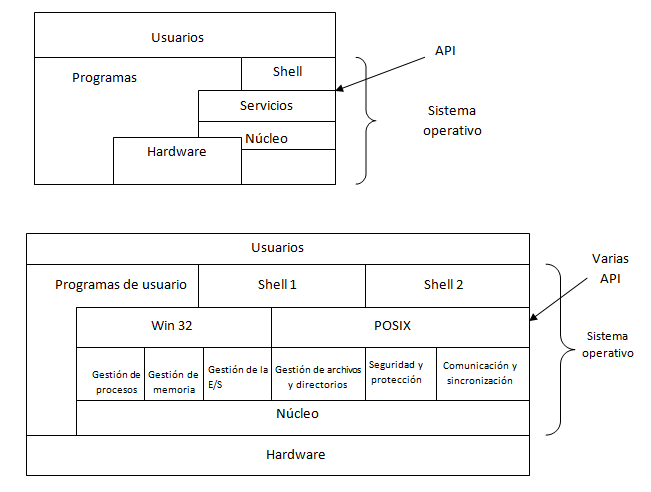
\includegraphics[width=0.9\textwidth]{./debuxos/unid.png}
\label{servizos}
\end{center}
\end{figure}

\begin{diapo} \begin{frame}{O servizo que remata un proceso é   \dots} 
\begin{enumerate}
	\item xestor de procesos\pause
	\item xestor de memoria \pause
	\item xestor de E/S 
\end{enumerate} \end{frame}  \end{diapo}  
%parella
\begin{diapo}\begin{frame}{ Se o micrófono non está conectado esta información manéxaa   \dots}
\begin{enumerate}
	\item xestor de procesos\pause
	\item xestor de memoria \pause
	\item xestor de E/S 
\end{enumerate} \end{frame} \end{diapo}

\begin{diapo} \begin{frame}{ A capa máis cercana ó hardware é  \dots} 
\begin{enumerate}
	\item kernel\pause
	\item software \pause
	\item malware 
\end{enumerate} \end{frame}  \end{diapo}  
%parella
\begin{diapo}\begin{frame}{ As API situaríanse na capa de   \dots}
\begin{enumerate}
	\item usuarios \pause
	\item xestión de arquivos \pause
	\item ningunha é correcta 
\end{enumerate} \end{frame} \end{diapo}

